


\section{Effect of other wave condition}
\label{sec: WC2 captive}

In this section the effect of the design optima is studied when the exact same breakwaters are interacting with Wave Condition 2: regular waves with a wave height of 9 metres and a peak period of 10.4 seconds. The exact same design space is used as in the first design iteration of Wave Condition 1 (Section \ref{sec: design iteration 1 captive}), so it also possesses the same factor boundaries as shown in Table \ref{tab: boundaries DI1 captive}. The performance of the 94 breakwaters is discussed in Section \ref{sec: DI1 captive H9 performance bw} and in Section \ref{sec: H9 captive correlation} correlations between factors and responses are mentioned. Finally, the design optima are shown in \ref{sec: H9 captive design optima}. 





\subsection{Performance breakwaters}
\label{sec: DI1 captive H9 performance bw}

The performance is again judged by plotting the wave transmission coefficient with respect to the mean wave drift fore of the structure. This forms a Pareto front, from which the best performing at attenuating wave energy large box-type breakwater around the water surface. Furthermore, a large wedge-type breakwater with a radius of 950 m, with a width of 120 m, a depth of 9.8 m, and a draught of 6.5 m performed well in wave attenuation. The two breakwaters that perform well at minimising the mean wave drift force are again box-type breakwaters relatively deeply submerged and a large breakwater with a large sloping beach at the wave-ward side. 

\begin{figure}[h]
    \centering
    \begin{subfigure}[b]{0.49\textwidth}
        \centering
        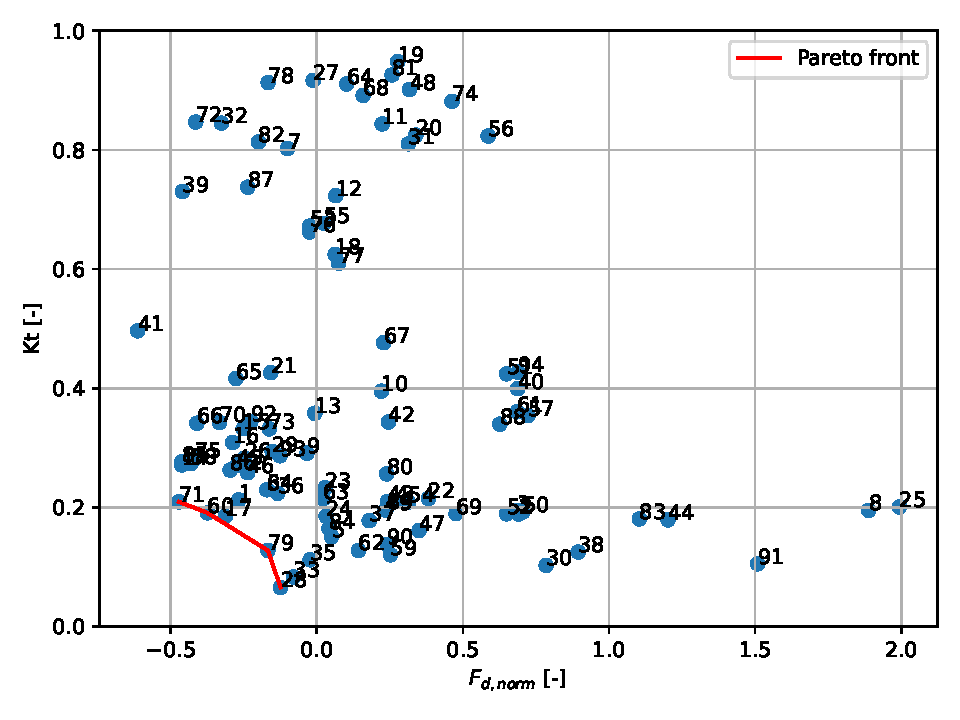
\includegraphics[width=\linewidth]{figures/ComFLOW/Results DI1 WC2 captive/Fd_norm_VS_Kt_normal.pdf}
        \caption[]%
        {{\small All breakwaters}}    
        \label{fig: Fd vs. Kt DI1 H9 captive normal}
    \end{subfigure}
    \hfill
    \begin{subfigure}[b]{0.49\textwidth}  
        \centering 
        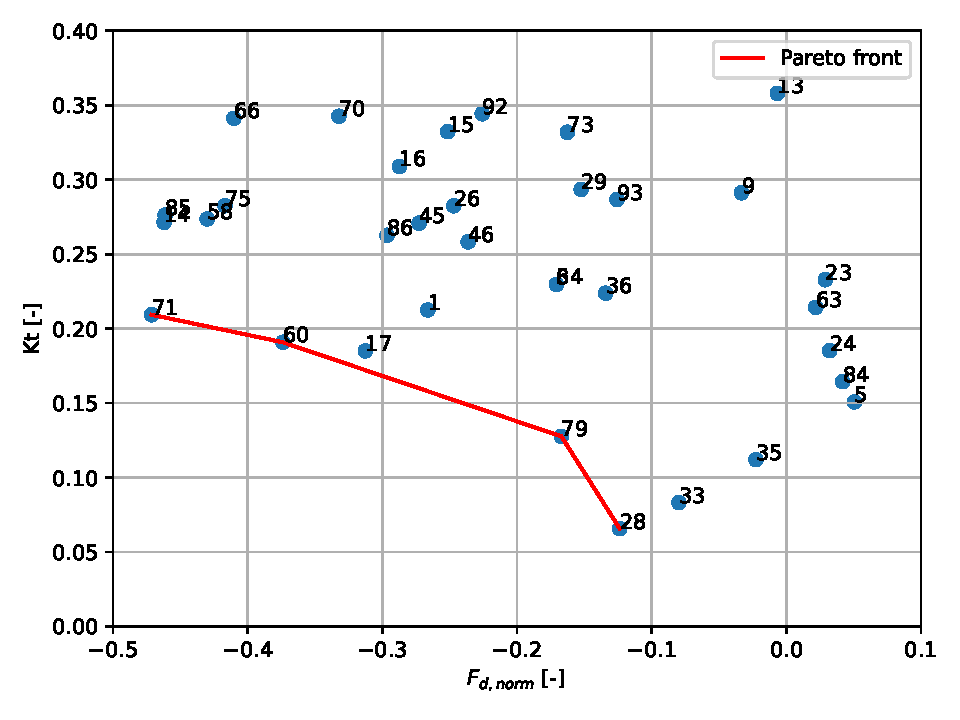
\includegraphics[width=\linewidth]{figures/ComFLOW/Results DI1 WC2 captive/Fd_norm_VS_Kt_Pareto.pdf}
        \caption[]%
        {{\small Pareto front}}    
        \label{fig: Fd vs. Kt DI1 H9 captive pareto}
    \end{subfigure}
    
    \caption{Mean wave drift force vs. Wave transmission}
    \label{fig: Fd vs. Kt DI1 H9 captive}
\end{figure}




\begin{figure}[h]
    \centering
    \begin{subfigure}[b]{0.49\textwidth}
        \centering
        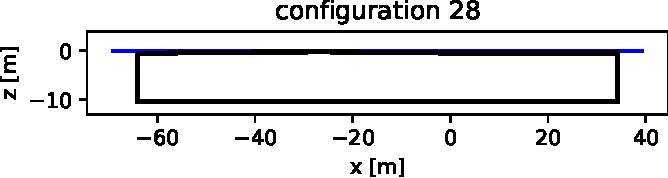
\includegraphics[width=\linewidth]{figures/ComFLOW/Breakwater Geometries/Design Iteration 1 captive WC2/breakwater_geometry28.pdf}
        \caption[]%
        {{\small }}    
        \label{}
    \end{subfigure}
    \hfill
    \begin{subfigure}[b]{0.49\textwidth}  
        \centering 
        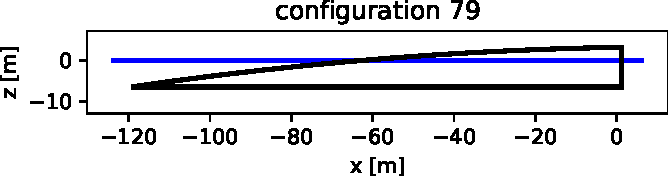
\includegraphics[width=\linewidth]{figures/ComFLOW/Breakwater Geometries/Design Iteration 1 captive WC2/breakwater_geometry79.pdf}    
        {{\small }}    
        \label{}
    \end{subfigure}
    
    \centering
    \begin{subfigure}[b]{0.49\textwidth}  
        \centering 
        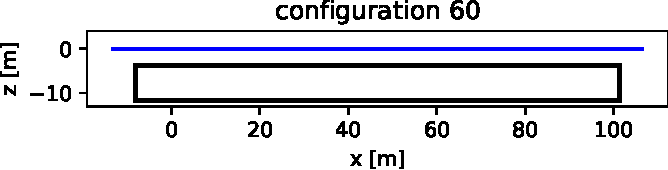
\includegraphics[width=\linewidth]{figures/ComFLOW/Breakwater Geometries/Design Iteration 1 captive WC2/breakwater_geometry60.pdf}    
        \caption[]%
        {{\small }}    
        \label{}
    \end{subfigure}
    \hfill
    \begin{subfigure}[b]{0.49\textwidth}
        \centering
        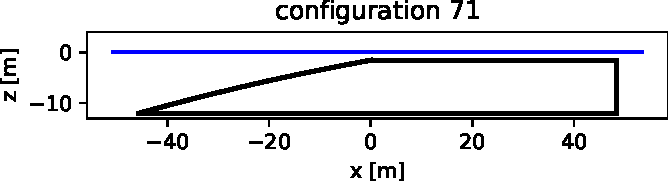
\includegraphics[width=\linewidth]{figures/ComFLOW/Breakwater Geometries/Design Iteration 1 captive WC2/breakwater_geometry71.pdf}    
        \caption[]%
        {{\small }}    
        \label{}
    \end{subfigure}
    
    \caption{Wave breakers on Pareto front}
    \label{}
\end{figure}




\subsection{Correlation}
\label{sec: H9 captive correlation}

Figure \ref{fig: correlation H9 DI1 captive} shows the correlation between all factors and responses. A clear negative correlation is visible between the mean wave drift force and factor F (WL), which can also be observed in Figure \ref{fig: Fd_norm_VS_top_bw_with_Kt H9 captive}. The same trend is visible as with Wave Condition 1, but for Wave Condition 2 the minimum WL is lower (i.e., minimal mean wave drift force experienced when breakwater is placed deeper in comparison with Wave Condition 1).  What can also be observed is a strong negative correlation between the transmission coefficient and factor B (floater width $W$). This was less present with Wave Condition 1. How this is possible is discussed in the last section of this chapter, in \ref{sec: hydro analysis wave transmission}.

\begin{figure}[h]
    \centering
    \begin{subfigure}[b]{0.34\textwidth}
        \centering
        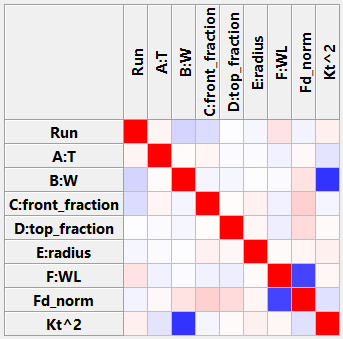
\includegraphics[width=\textwidth]{figures/ComFLOW/Results DI1 WC2 captive/correlation_H9.png}
        \caption[]%
        {{\small Correlation between factors and responses}}    
        \label{fig: correlation H9 DI1 captive}
    \end{subfigure}
    \hfill
    \begin{subfigure}[b]{0.49\textwidth}
        \centering 
        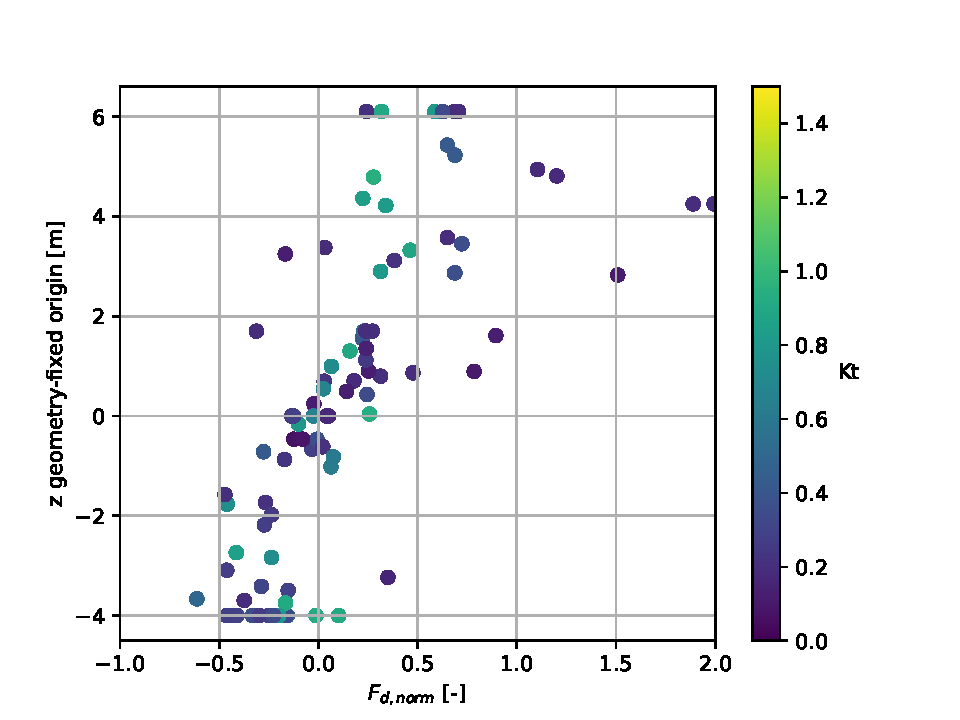
\includegraphics[width=\textwidth]{figures/ComFLOW/Results DI1 WC2 captive/Fd_norm_VS_top_bw_with_Kt.pdf}
        \caption[]%
        {{\small Mean wave drift force to z-positioning breakwaters}}    
        \label{fig: Fd_norm_VS_top_bw_with_Kt H9 captive}
    \end{subfigure}

    \caption{}
    \label{fig: }
\end{figure}




\subsection{Design Optima}
\label{sec: H9 captive design optima}

\subsubsection{Based on minimal mean wave drift force}
All optima possess a sloping beach, while with Wave Condition 1 shallow box-type optima were given. The configurations are placed around 2.8 metres beneath the waterline. The floater width converged to around 95 metres, and the depth to 7.6 metres.


% \usepackage{booktabs}
\begin{table}[h]
\centering
\scalebox{0.65}{
\begin{tabular}{@{}ccccccccccc@{}}
\toprule
configuration & T        & W        & front\_fraction & top\_fraction & radius   & WL & $F_{d,norm,DoE}$ & $K_{t,DoE}^2$  & $F_{d,norm,ComFLOW}$  & $K_{t,ComFLOW}^2$      \\ \midrule
1  & 7.629 & 95.858 & 0.010 & 0.832 & 1999.982 & 2.864 & -1.015 & 0.043 & -0.61 & 0.21\\
2  & 7.512 & 93.288 & 0.010 & 0.821 & 1999.992 & 2.753 & -1.014 & 0.039 \\
3  & 7.505 & 91.023 & 0.010 & 0.844 & 1995.183 & 2.889 & -1.013 & 0.039 \\
4  & 7.714 & 84.492 & 0.010 & 0.845 & 1999.997 & 2.799 & -1.012 & 0.032 \\
5  & 8.681 & 90.079 & 0.010 & 0.829 & 1999.997 & 2.809 & -1.010 & 0.034 \\
6  & 8.132 & 92.114 & 0.017 & 0.832 & 1999.999 & 2.853 & -1.008 & 0.038 \\
7  & 5.928 & 92.438 & 0.011 & 0.863 & 1999.996 & 2.756 & -1.004 & 0.044 \\
8  & 7.288 & 99.293 & 0.010 & 0.778 & 1999.997 & 2.961 & -1.002 & 0.053 \\
9  & 9.059 & 96.508 & 0.011 & 0.835 & 2000.000 & 2.738 & -1.002 & 0.042 \\
10 & 9.471 & 92.380 & 0.010 & 0.817 & 1999.998 & 3.017 & -0.997 & 0.045 \\ \\ \bottomrule


\end{tabular}
}
\caption{Parameters optimal breakwaters based on minimal mean wave drift force}
\label{tab: params design iteration 1 captive br 1to10}
\end{table}

\begin{figure}[h]
    \centering
    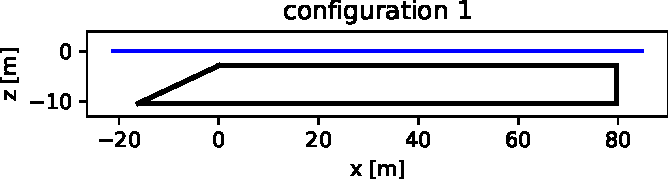
\includegraphics[width=0.475\textwidth]{figures/ComFLOW/Breakwater Geometries/Design Iteration 1 captive/DI1-WC2 captive/breakwater_geometry1_Fd.pdf}
    \caption{The most optimal breakwaters based on minimal mean wave drift force}
    \label{fig:  most optimal breakwaters DI2 Fd}
\end{figure}







\subsubsection{Based on minimal transmission coefficient}
Various optima were given based on the minimal transmission coefficient. Again, they are placed closer to or even partly above the waterline. But those crossing the waterline are expected to have a relatively high mean wave drift force. 



% \usepackage{booktabs}
\begin{table}[h]
\centering
\scalebox{0.65}{
\begin{tabular}{@{}ccccccccccc@{}}
\toprule
configuration & T        & W        & front\_fraction & top\_fraction & radius   & WL & $F_{d,norm,DoE}$ & $K_{t,DoE}^2$  & $F_{d,norm,ComFLOW}$  & $K_{t,ComFLOW}^2$      \\ \midrule
1  & 10.613 & 141.962 & 0.693 & 0.817 & 1238.764 & -0.835 & 0.475  & -0.010 & 0.15 & 0.06\\
2  & 9.837  & 144.817 & 0.958 & 0.099 & 1897.583 & 1.012  & -0.030 & -0.010 \\
3  & 9.458  & 94.390  & 0.937 & 0.079 & 502.282  & -3.484 & 1.378  & -0.001 \\
4  & 8.151  & 90.276  & 0.868 & 0.920 & 519.186  & -2.074 & 0.620  & -0.006 \\
5  & 10.950 & 147.716 & 0.553 & 0.478 & 1185.615 & -0.180 & 0.194  & -0.025 \\
6  & 10.022 & 134.414 & 0.435 & 0.377 & 1414.444 & -2.978 & 0.961  & -0.001 \\
7  & 8.864  & 146.746 & 0.612 & 0.956 & 1744.526 & -2.528 & 1.309  & -0.025 \\
8  & 6.889  & 149.836 & 0.976 & 0.985 & 586.127  & -5.268 & 1.009  & -0.001 \\
9  & 10.191 & 100.066 & 0.905 & 0.423 & 1322.430 & -1.802 & 0.637  & -0.004 \\
10 & 3.046  & 97.343  & 0.073 & 0.049 & 1891.990 & 1.120  & -0.199 & -0.001  \\ \bottomrule


\end{tabular}
}
\caption{Parameters optimal breakwaters based on minimal transmission coefficient}
\label{tab: params design iteration 1 captive br 1to10}
\end{table}

\begin{figure}[h]
    \centering
    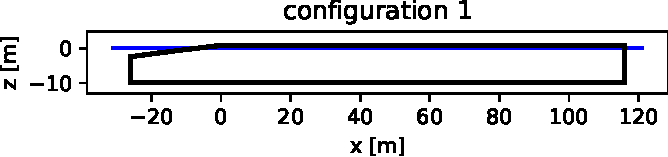
\includegraphics[width=0.475\textwidth]{figures/ComFLOW/Breakwater Geometries/Design Iteration 1 captive/DI1-WC2 captive/breakwater_geometry1_Kt.pdf}
    \caption{The most optimal breakwaters based on minimal transmission coefficient}
    \label{fig:  most optimal breakwaters DI2}
\end{figure}




\section{Effect of motion allowance}
Another optimisation is done for moving structures, where the breakwater can translate in x-direction and rotate in pitch direction within the xz-plane around its connection point with the floating island. Due to a bug in the software, some simulations were moving in an unrealistic way and many of these simulations became unstable after some time. The data of these simulations could not be trusted enough to perform a proper design optimisation. But, with the data that were useful, the following plots are made. The most interesting observation is that the same trend as with the captive design optimisation is visible, but the correlation is much weaker. Many of the submerged breakwaters experience a positive mean wave drift force, while for the captive design optimisation, almost all submerged breakwaters had a negative mean wave load. This is expected because, when motions are allowed, the breakwater will move depending on the pressure field around the breakwater. For example, when a low pressure field is on the left side of the breakwater, the structure will move towards this low pressure field. Therefore, the low-pressure field will become smaller as the breakwater is intruding it. Because the force on the object is directly related to the pressure around the structure, this will significantly influence the mean wave drift force.

\begin{figure}[h]
    \centering
    \begin{subfigure}[b]{0.49\textwidth}
        \centering
        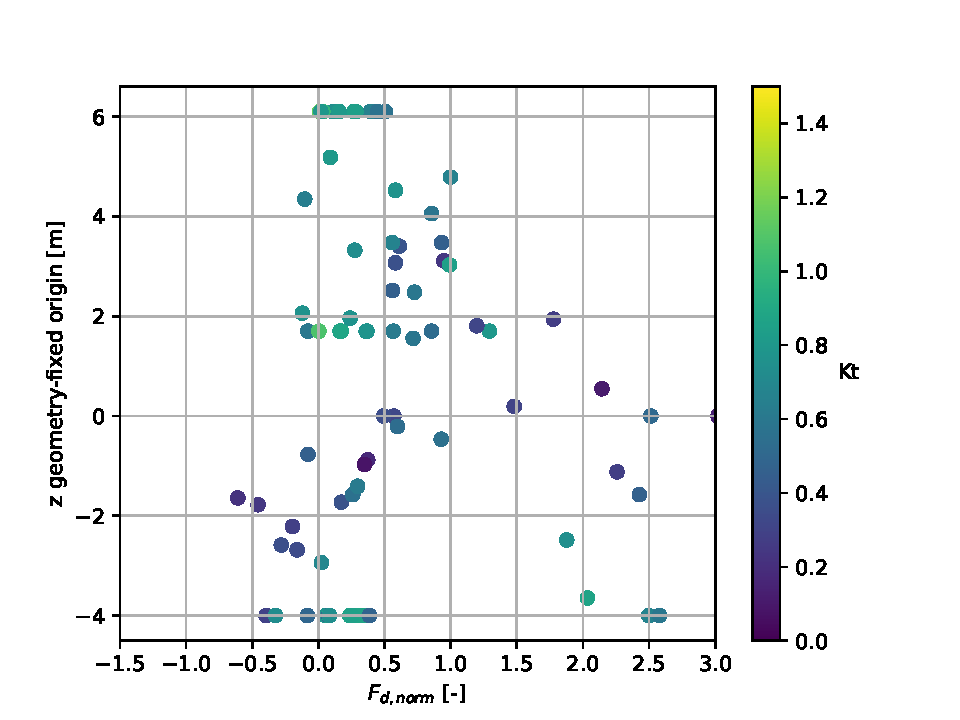
\includegraphics[width=\linewidth]{figures/ComFLOW/Results moving/DI1/H3/Fd_norm_VS_top_bw_with_Kt.pdf}
        \caption[]%
        {{\small Wave Condition 1: H = 3.0 m and T = 6.0 s}}    
        \label{fig: Fd_norm_VS_top_bw_with_Kt DI1 H3 moving}
    \end{subfigure}
    \hfill
    \begin{subfigure}[b]{0.49\textwidth}
        \centering
        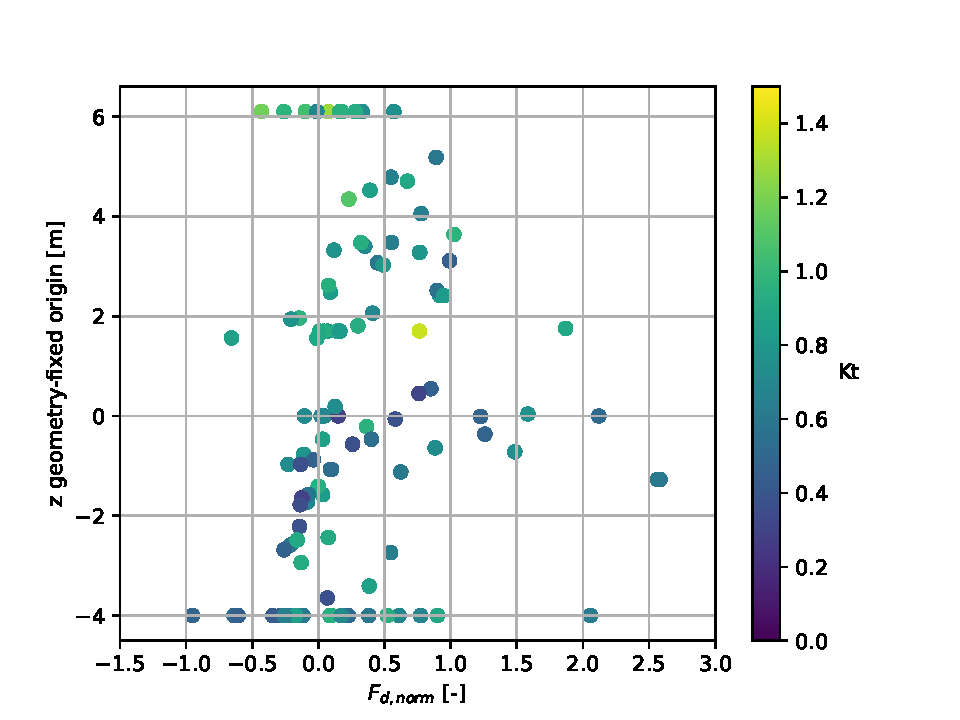
\includegraphics[width=\linewidth]{figures/ComFLOW/Results moving/DI1/H9/Fd_norm_VS_top_bw_with_Kt.pdf}
        \caption[]%
        {{\small Wave Condition 2: H = 9.0 m and T = 10.4 s}}    
        \label{fig: Fd_norm_VS_top_bw_with_Kt DI1 H9 moving}
    \end{subfigure}
    
    \caption{Mean wave drift force dependent on their z-positioning of moving breakwaters}
    \label{fig: }
\end{figure}


